\documentclass{article}
\usepackage[utf8]{inputenc}
\usepackage[margin=1in,includefoot]{geometry}

% Header and Footer Setup
\usepackage{fancyhdr}
\pagestyle{fancy}
\fancyhead{}
\fancyfoot{}
\fancyfoot[R]{\thepage}
\renewcommand{\headrulewidth}{0pt}
\renewcommand{\footrulewidth}{0pt}
%
%Graphics Setup
\usepackage{graphicx}
\usepackage{float}
\usepackage{subfig}

%list setup
\usepackage{amssymb}
\renewcommand{\labelitemi}{$\blacktriangleright$}
\renewcommand{\labelitemii}{$\bullet$}
\renewcommand{\labelitemiii}{$\circ$}



%Source Code setup
\usepackage{xcolor}
\usepackage{listings}

\definecolor{mGreen}{rgb}{0,0.6,0}
\definecolor{mGray}{rgb}{0.5,0.5,0.5}
\definecolor{mPurple}{rgb}{0.58,0,0.82}
\definecolor{backgroundColour}{rgb}{0.95,0.95,0.92}

\lstdefinestyle{CStyle}{
    backgroundcolor=\color{backgroundColour},   
    commentstyle=\color{mGreen},
    keywordstyle=\color{magenta},
    numberstyle=\tiny\color{mGray},
    stringstyle=\color{mPurple},
    basicstyle=\footnotesize,
    breakatwhitespace=false,         
    breaklines=true,                 
    captionpos=b,                    
    keepspaces=true,                 
    numbers=left,                    
    numbersep=5pt,                  
    showspaces=false,                
    showstringspaces=false,
    showtabs=false,                  
    tabsize=2,
    language=C
}
%


\begin{document}

\begin{titlepage}

	\begin{flushright}
	\textsc{\large May 29, 2021} \\
	\end{flushright}
	\begin{center}
	\Large{\bfseries GTU Department of Computer Engineering \\ CSE312/CSE504 - Spring 2021 \\ Homework 2 Report  } \\
	\end{center}
	\topskip0pt
	\vspace*{\fill}
	\begin{center}
	\Large{\bfseries Akif Kartal \\ 171044098 }
	\end{center}
	\vspace*{\fill}

\end{titlepage}

\cleardoublepage
\section{Problem Definition}
The problem is to implement a kernel that will support multi- threading, interrupt handling and inter-process
communication in SPIM simulator.

\section{Solution}
In order to solve this problem first we need to implement\textbf{ required system calls} for this problem. 

\subsection{System Calls}
\subsubsection{Create Thread Syscall}
In order to create thread correct way we need to this syscall.\\ \\
Assembly Test File;
\begin{figure}[H]
    \centering
	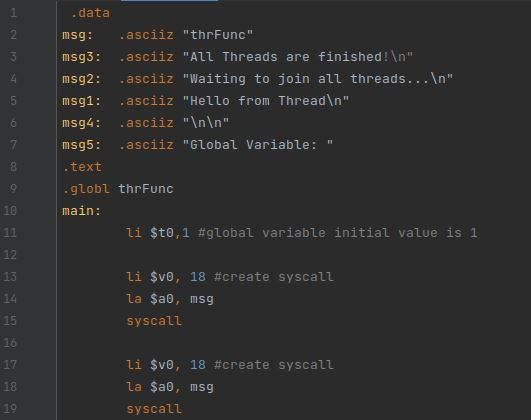
\includegraphics[width=6in, height=4.5in]{11.JPG}
	\caption[Optional caption]{}
	\label{}
\end{figure}
\cleardoublepage
Output;
\begin{figure}[H]
    \centering
	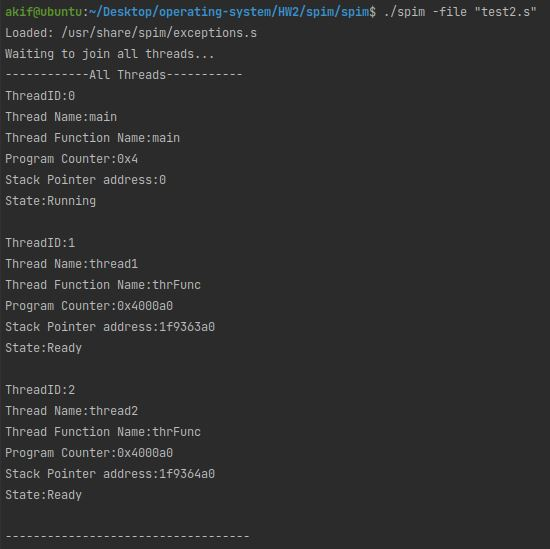
\includegraphics[width=6in, height=4.5in]{9.JPG}
	\caption[Optional caption]{}
	\label{}
\end{figure}

\subsubsection{Join Thread Syscall}
In order to join thread correct way we need to this syscall. My Join syscal is waiting all thread to be finished.\\ \\
Assembly Test File;
\begin{figure}[H]
    \centering
	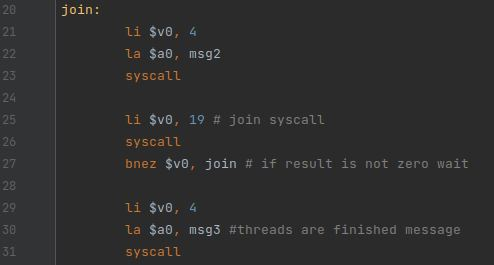
\includegraphics[width=5in, height=5.5in]{12.JPG}
	\caption[Optional caption]{}
	\label{}
\end{figure}
\subsubsection{Exit Thread Syscall}
In order to join thread correct way we need to this syscall. \\ \\
Assembly Test File;
\begin{figure}[H]
    \centering
	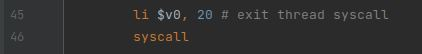
\includegraphics[width=6in, height=0.8in]{13.JPG}
	\caption[Optional caption]{}
	\label{}
\end{figure}       
\cleardoublepage                       
\subsubsection{Combine All Syscall}
We have implemented required system calls. In following test we will test these by incrementing a global variable which is shared between all threads. \\ \\
Following two picture contains test file assembly codes; 
\begin{figure}[H]
    \centering
    \subfloat[\centering first half of code]{{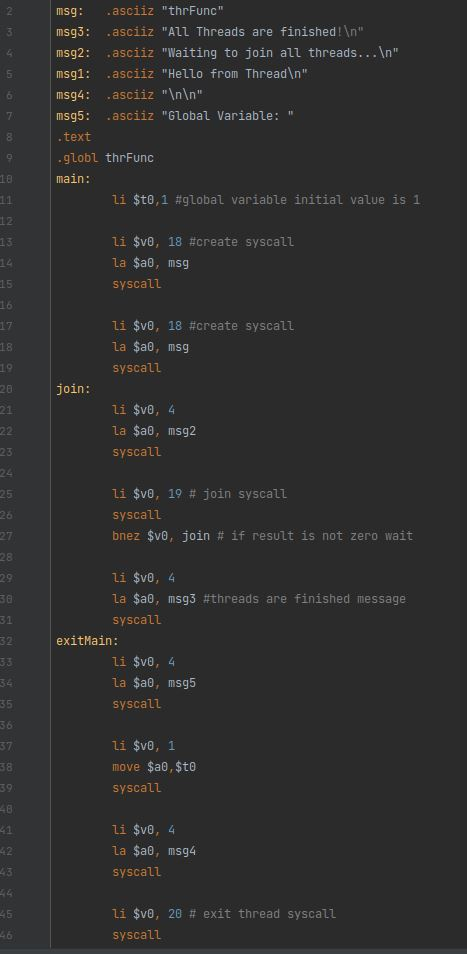
\includegraphics[width=7cm,height=6.5in]{7.JPG} }}%
    \qquad
    \subfloat[\centering other half]{{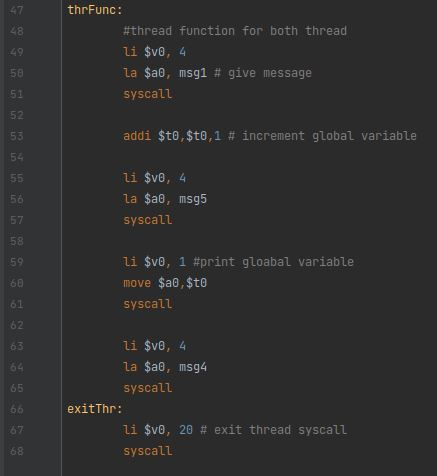
\includegraphics[width=8cm,height=6.5in]{8.JPG} }}%
    
\end{figure} 
\cleardoublepage 
\textbf{Test Results} \\ \\
\begin{figure}[H]
    \centering
    \subfloat[\centering first half of result]{{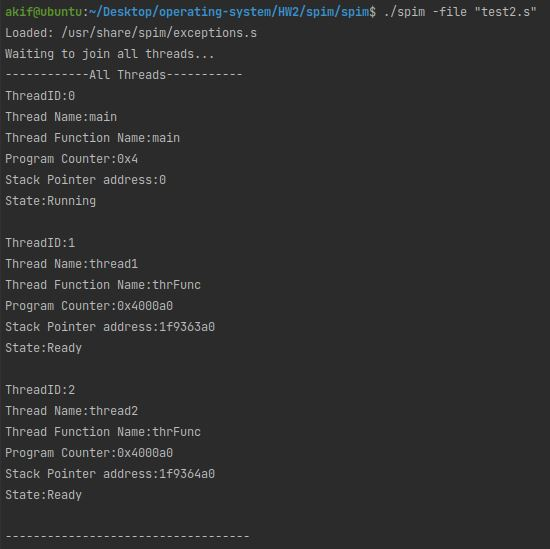
\includegraphics[width=8cm,height=6in]{9.JPG} }}%
    \qquad
    \subfloat[\centering other half]{{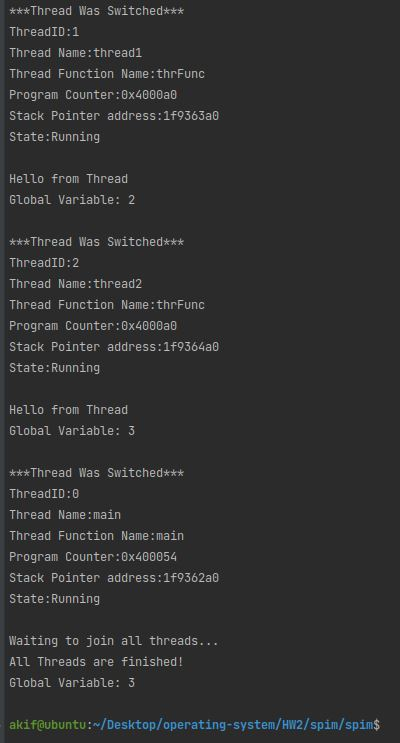
\includegraphics[width=7cm,height=6in]{10.JPG} }}%
    
\end{figure} 
In this test, context switch was made by using \textbf{Round Robin scheduling algorithm} as can be seen in result. \\ \\
Also, since thread function is very simple in this test there was no timer interrupt.
\cleardoublepage 
\section{Problems}
\subsection{Producer Consumer Problem}
In this problem we have two different version first is without mutex and second is with mutex.In this test buffer is a variable only not an array
\subsubsection{Without Mutex}
In this version we will not use mutex and we will show that there is a race condition. \\ \\
\textbf{Main Thread assembly Code;} \\
\begin{figure}[H]
    \centering
    \subfloat[\centering first half of code]{{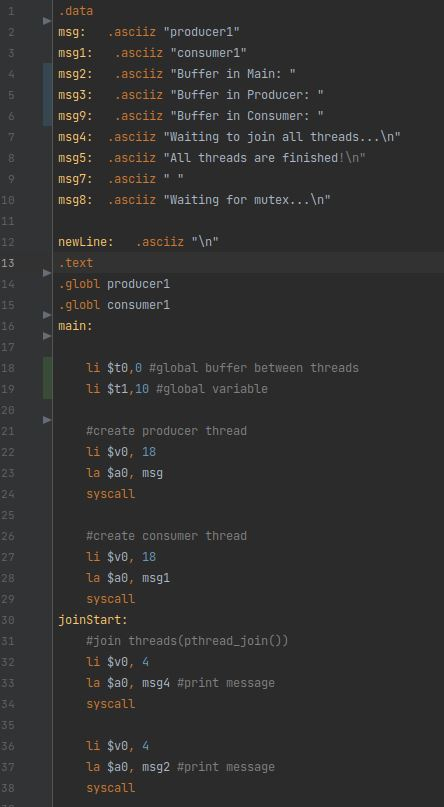
\includegraphics[width=7cm,height=5.5in]{14.JPG} }}%
    \qquad
    \subfloat[\centering other half]{{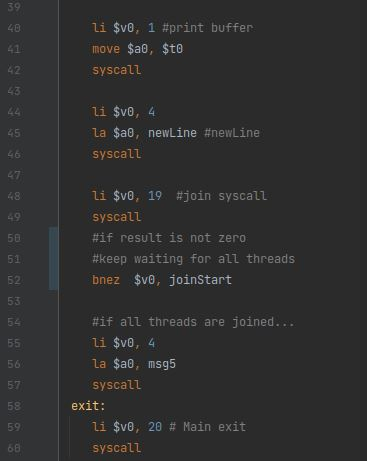
\includegraphics[width=7cm,height=5.5in]{15.JPG} }}%
    
\end{figure} 
\cleardoublepage 
\textbf{Other Threads assembly Code(no mutex yet!);} \\
\begin{figure}[H]
    \centering
    \subfloat[\centering Producer Thread]{{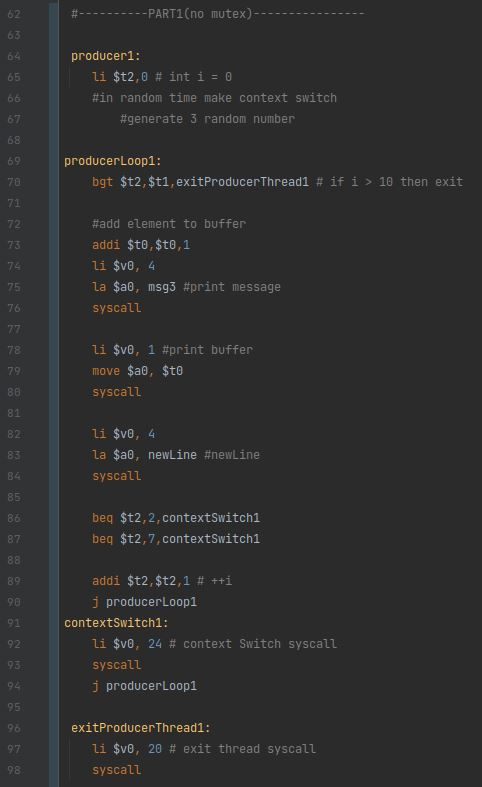
\includegraphics[width=7cm,height=6in]{16.JPG} }}%
    \qquad
    \subfloat[\centering Consumer Thread]{{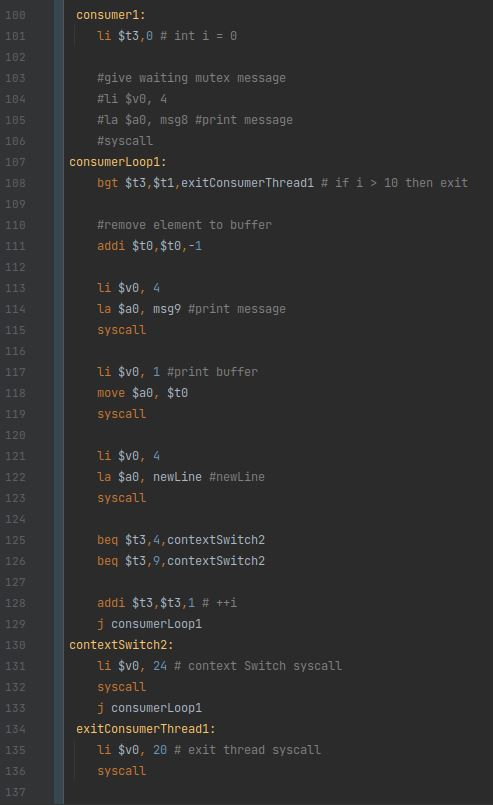
\includegraphics[width=7cm,height=6in]{17.JPG} }}%
    
\end{figure} 
\textbf{What are we doing in this test?} \\ \\
In this test we have a global buffer and producer is incrementing it, also consumer is decrementing it. But, while doing this in both
producer and consumer threads we are making 2 times context switch by using a context switch syscall in order to simulate real problem. Lastly,
we are printing buffer's situation in all threads(main,producer,consumer). Check the following test results to see race condition.
\cleardoublepage 
\textbf{Test Results (no mutex yet!);} \\

\begin{figure}[H]
    \centering
	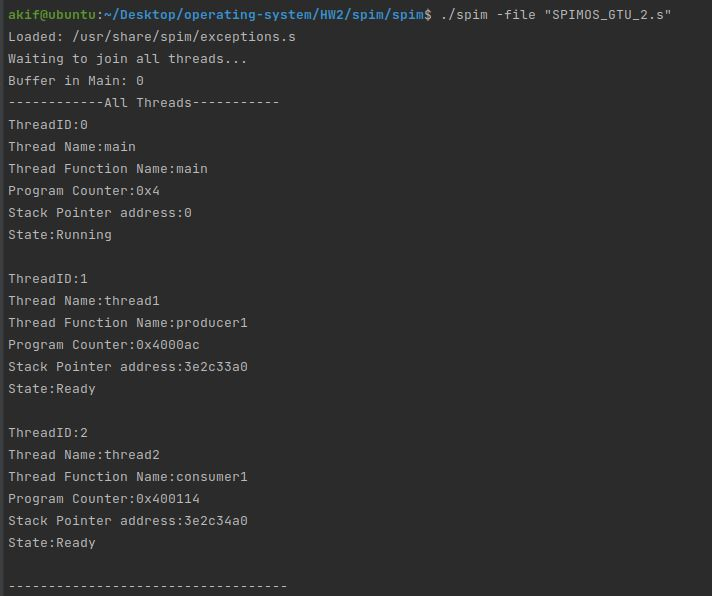
\includegraphics[width=5in, height=5.5in]{18.JPG}
	\caption[Optional caption]{All Threads in program}
	\label{}
\end{figure}
\hfill \break
As you can see buffer is 0 at the beginning of the program. Let see thread switching and race conditions.
\cleardoublepage
\begin{figure}[H]
    \centering
    \subfloat[\centering Half of test result]{{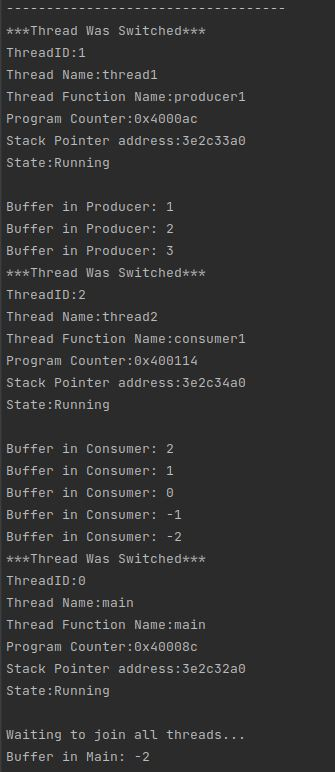
\includegraphics[width=7cm,height=6in]{19.JPG} }}%
    \qquad
    \subfloat[\centering other half after a few context switch]{{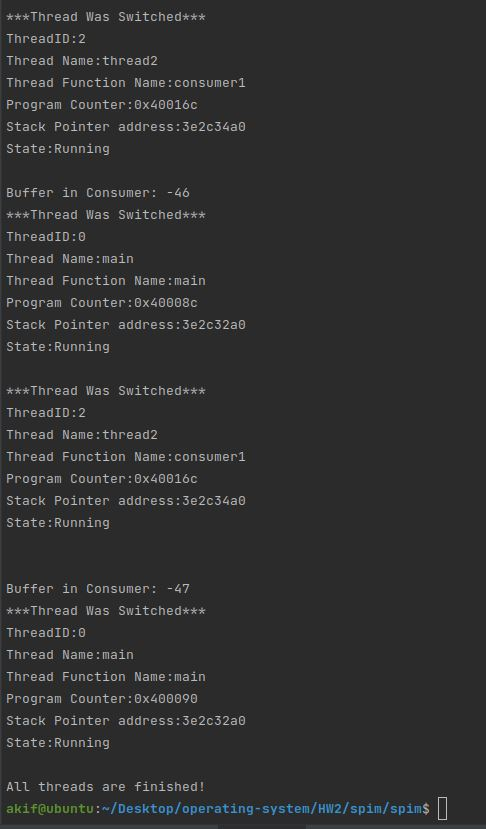
\includegraphics[width=7cm,height=6in]{20.JPG} }}%    
\end{figure} 
\hfill \break
\hfill \break
As you can see from test result buffer start with 0 but finished with -47. Since there is a race condition ,we don't know which
thread will run how many times. Now \textbf{we have showed the race condition}. Lets look at the with mutex version.
\cleardoublepage
\subsubsection{With Mutex}
In this version we will use mutex and we will show that there is no race condition. \\ \\
\textbf{Main Thread assembly Code} \\
\begin{figure}[H]
    \centering
    \subfloat[\centering first half of code]{{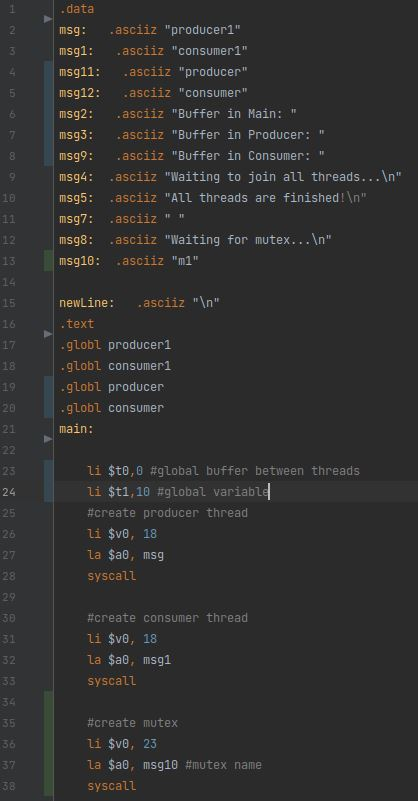
\includegraphics[width=7cm,height=5.5in]{30.JPG} }}%
    \qquad
    \subfloat[\centering other half]{{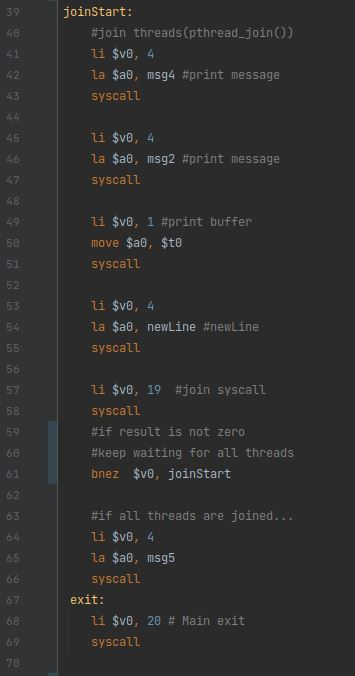
\includegraphics[width=7cm,height=5.5in]{31.JPG} }}%
    
\end{figure} 
\cleardoublepage 
\textbf{Other Threads assembly Code} \\
\begin{figure}[H]
    \centering
    \subfloat[\centering Producer Thread]{{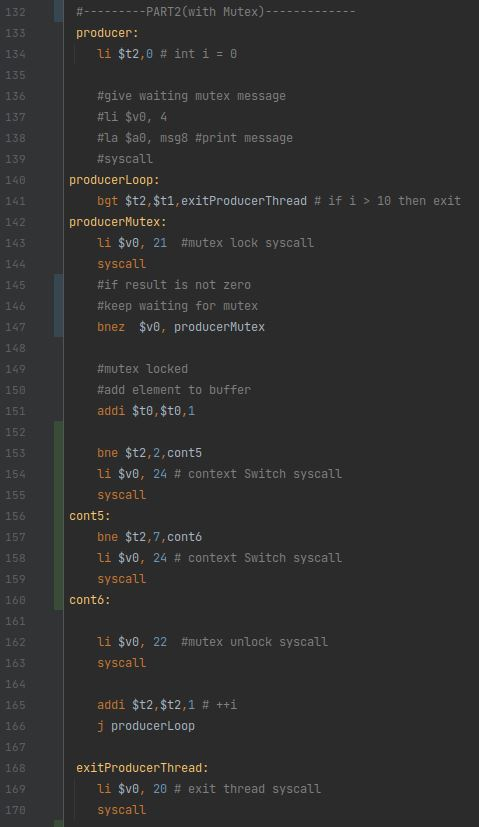
\includegraphics[width=7cm,height=6in]{32.JPG} }}%
    \qquad
    \subfloat[\centering Consumer Thread]{{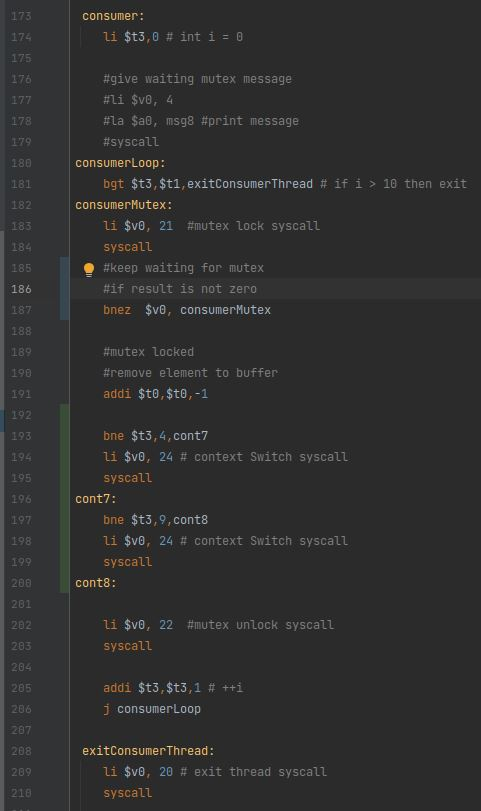
\includegraphics[width=7cm,height=6in]{33.JPG} }}%
    
\end{figure}
\hfill \break 
As in one before test, as a buffer we are only incrementing and decrementing a global variable in this test.
\cleardoublepage 
\textbf{Test Results} \\

\begin{figure}[H]
    \centering
	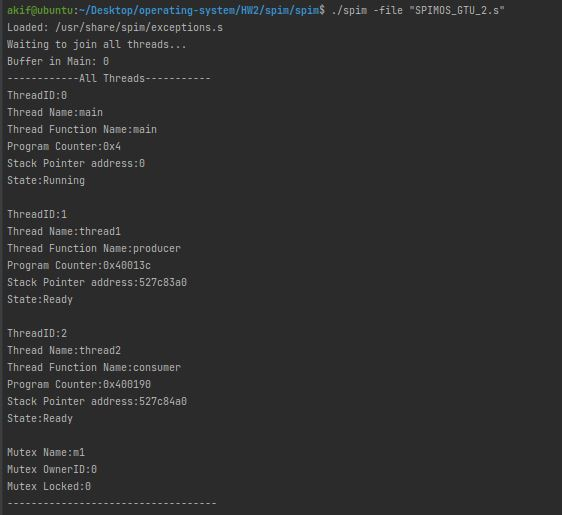
\includegraphics[width=5in, height=5.5in]{24.JPG}
	\caption[Optional caption]{All Threads and Mutexes in program}
	\label{}
\end{figure}
\hfill \break
As you can see buffer is 0 at the beginning of the program. Let see thread switching and result.
\cleardoublepage
\begin{figure}[H]
    \centering
    \subfloat[\centering Half of test result]{{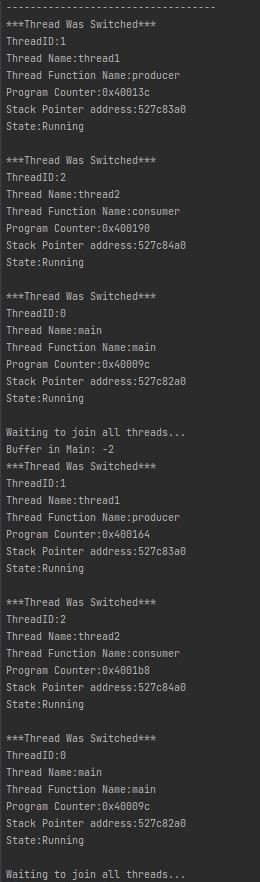
\includegraphics[width=7cm,height=7in]{25.JPG} }}%
    \qquad
    \subfloat[\centering other half after a few context switch]{{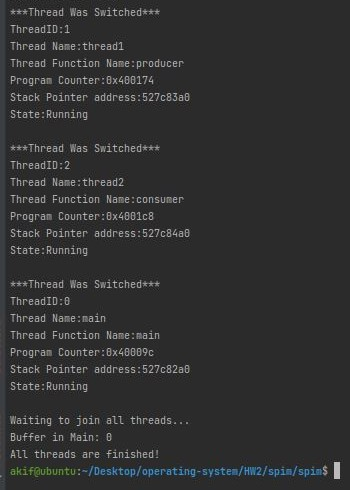
\includegraphics[width=7cm,height=7in]{26.JPG} }}%    
\end{figure} 
As a result since we have used mutex last result is 0 as expected.
\cleardoublepage
\subsection{Merge Sort with multi-threaded}
In this problem we will implement merge sort with using more than one thread. \\ \\
\textbf{Solution Steps}
\begin{itemize}
	\item First, implement multi-threaded merge sort in C++ and make sure it works correctly.
	\item Then, write multi-threaded merge sort in mips assembly by using C++ code.
	\item Test assembly file in spim and make sure it works.
\end{itemize}
\subsubsection{Multi-threaded merge sort in C++}
In homework pdf file given merge sort code \textbf{is not work} with different array and thread size. Then I found and corrected a working
multi-threaded merge sort in C++ code. Check following test results. \\ \\
\textbf{Simple Test Result} \\
\begin{figure}[H]
    \centering
	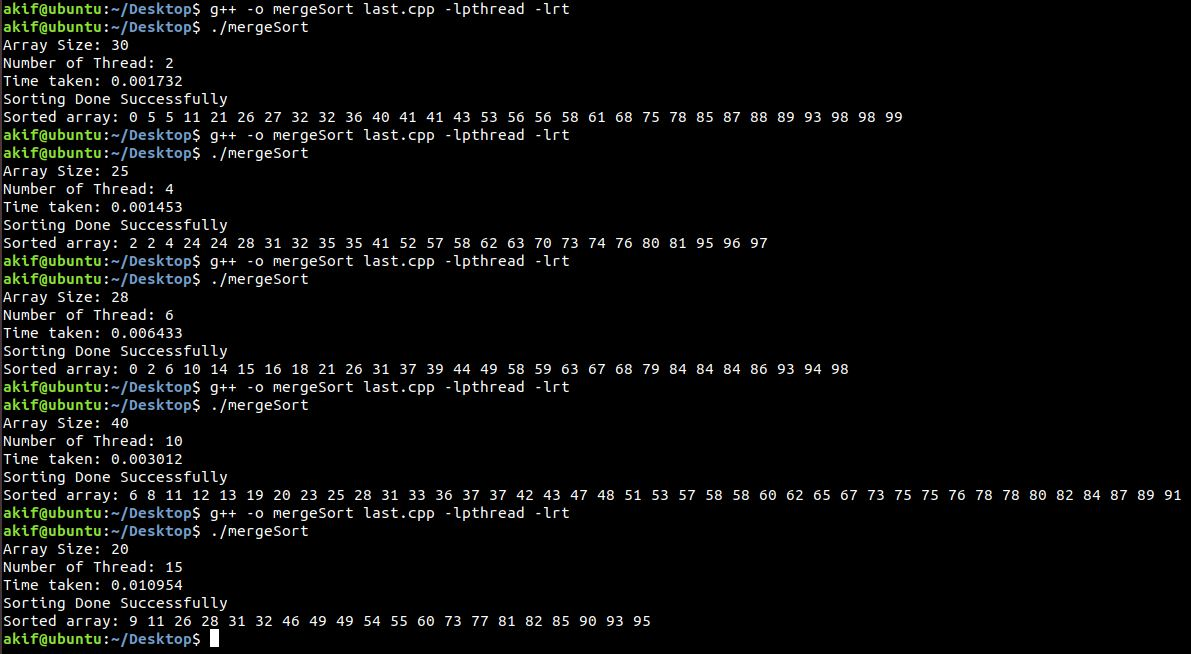
\includegraphics[width=7in, height=5in]{35.JPG}
	\caption[Optional caption]{Multi-threaded merge sort in C++}
	\label{}
\end{figure}
\subsubsection{Multi-threaded merge sort in mips assembly}
I have implemented Multi-threaded merge sort in SPIMOS\_GTU\_1.s file as mips assembly by using my C++ code.
Check \textbf{SPIMOS\_GTU\_1.s} file to see code.
\subsubsection{Testing in SPIM}
Since, merge sort is a recursive algorithm it is difficult to implement recursive functions in assembly, you need to very careful,
because of this difficulty my assembly code \textbf{didn't work} in spim. I am creating threads \textbf{correctly} but I am getting some
program counter error because of \textbf{recursive functions} in merge sort algorithm. \\ \\
\textbf{My threads in merge Sort} 
\begin{figure}[H]
    \centering
	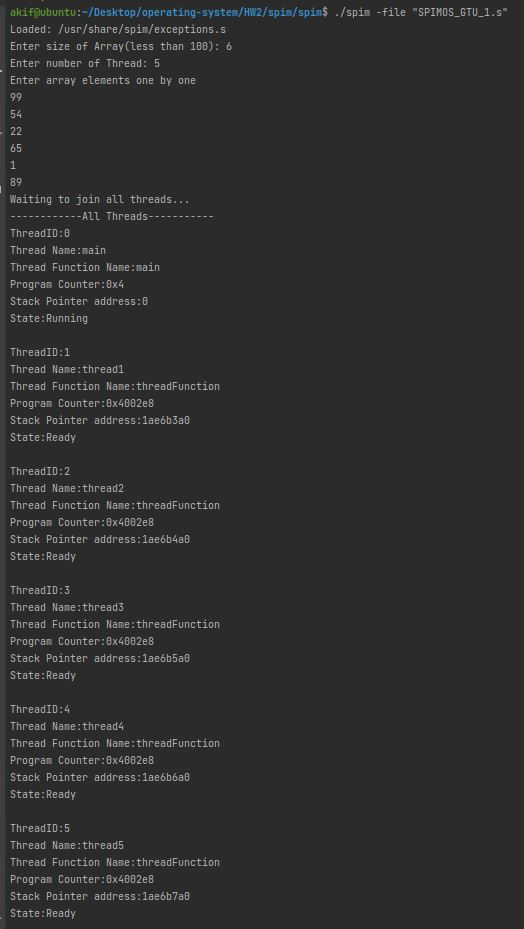
\includegraphics[width=5in, height=6in]{34.JPG}
	\caption[Optional caption]{Threads in merge Sort}
	\label{}
\end{figure}
\hfill \break
As you can see, we are creating threads correct way but after that because of recursive algorithms we are getting program counter errors which is
not happen in producer consumer problem. Thread function is merge function C++ code.
\section{Implementation Details in SPIM}
\begin{figure}[H]
    \centering
    \subfloat[\centering My syscalls in SPIM]{{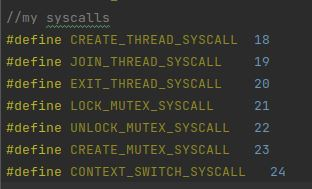
\includegraphics[width=7cm,height=2in]{36.JPG} }}%
    \qquad
    \subfloat[\centering My Data in SPIM]{{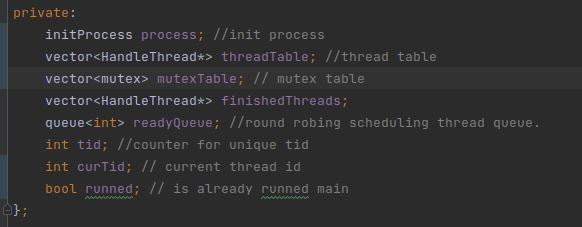
\includegraphics[width=7cm,height=2in]{37.JPG} }}%    
\end{figure} 



 




\end{document}